% scatterplot.tex
\documentclass[tikz]{standalone}
\usepackage{pgfplots}

\begin{document}
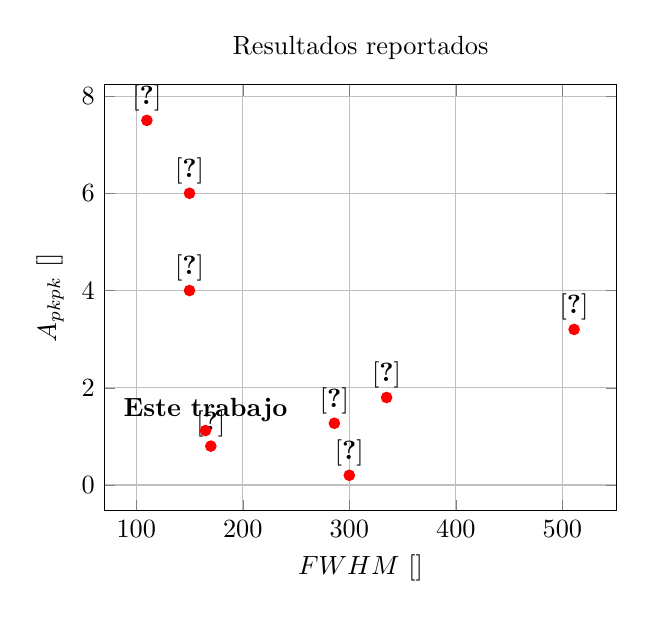
\begin{tikzpicture}[scale=0.95]
  \begin{axis}[
    xlabel={$FWHM$ [\unit{\pico\second}]},
    ylabel={$A_{pkpk}$ [\unit{\volt}]},
    title=Resultados reportados,
    grid=both
    ]
    \addplot[
        scatter/classes={a={blue}, b={red}},
        scatter, mark=*, only marks, 
        scatter src=explicit symbolic,
        nodes near coords*={\Label},
        visualization depends on={value \thisrow{label} \as \Label} %<- added value
    ] table [meta=class] {
        x   y       class   label
        511 3.2     b       {\cite{rulikowski2004}}
        335 1.8     b       {\cite{rulikowski2004}}
        110 7.5     b       {\cite{protiva2009}}
        170 0.8     b       {\cite{kamal2014}}
        300 0.2     b       {\cite{han2002}}
        150 6       b       {\cite{han2005}}
        150 4       b       {\cite{han2005}}
        286 1.27    b       {\cite{oloumi2018}}
        165 1.12    b       {\textbf{Este trabajo}}
    };
  \end{axis}
\end{tikzpicture}
\end{document}
